\documentclass[numbers=noenddot,10pt,a4paper]{scrartcl}
\usepackage[greek,ngerman]{babel}
\usepackage[T1]{fontenc}
\usepackage[utf8]{inputenc}
\usepackage{fullpage}
\usepackage{libertine}
\usepackage{ziffer}
\usepackage{graphicx}
\usepackage{units}
%\usepackage{wasysym}
\usepackage{amsmath}
\usepackage{amssymb}
\usepackage{wrapfig}
\usepackage{esint}
\usepackage{float}
\usepackage{wrapfig}
\usepackage[font=small]{caption}
\usepackage{subcaption}

\renewcommand{\thefigure}{Abb. \arabic{figure}}

\captionsetup[wrapfigure]{name=}
\captionsetup[figure]{name=}
\newcommand{\degree}{^\circ}
\newcommand{\diff}{\textnormal{d}}
\newcommand{\tenpo}[1]{\cdot 10^{#1}}
\newcommand{\greek}[1]{\greektext#1\latintext}
\newcommand{\ix}[1]{_\text{#1}}

\title{Protokoll: Schmitt-Trigger}
\author{Tom Kranz, Philipp Hacker}
\date{\today}

\begin{document}
%\setcounter{page}{2}
%\setcounter{section}{1}
\maketitle
\vspace*{\fill}
\tableofcontents
\vfill
\newpage
\section{Vorbereitung}
\subsection{Schaltskizzen}
\begin{figure}[H]
\centering
\begin{subfigure}[b]{0.49\textwidth}
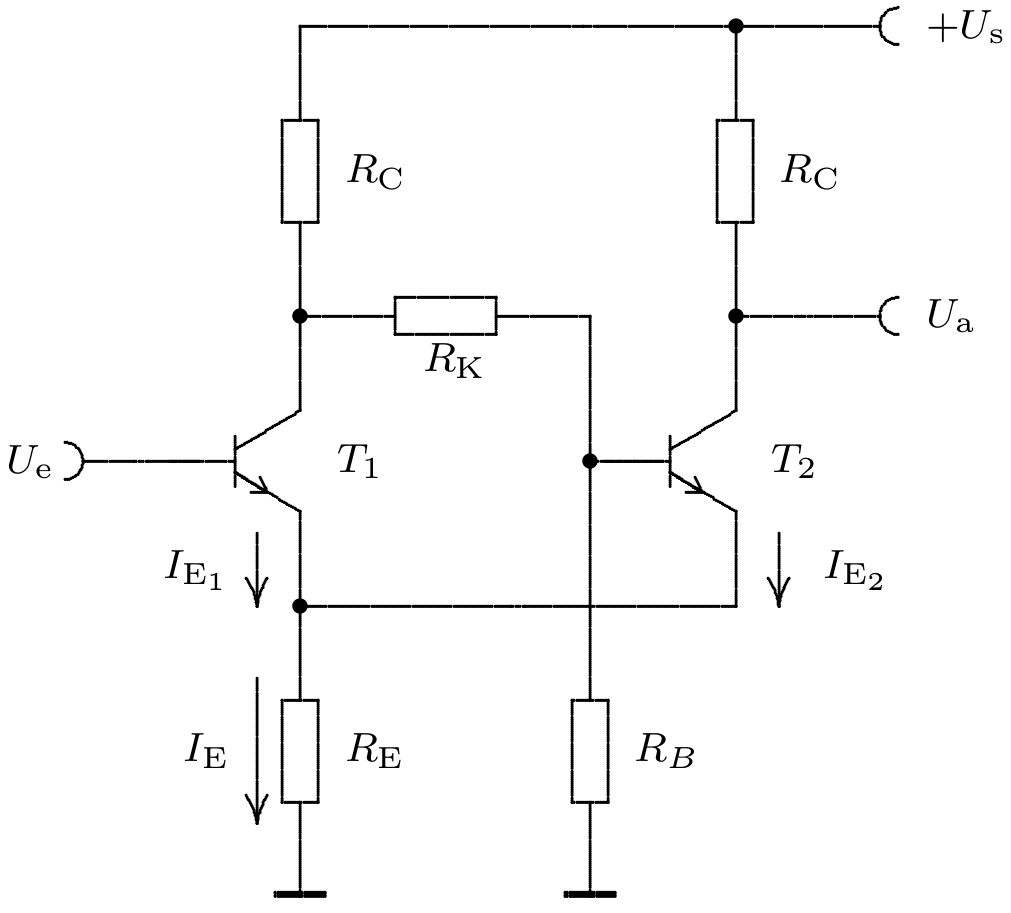
\includegraphics[width=\textwidth]{schaltskizze_st2.png}
\caption{Grundschaltung}
\end{subfigure}
\begin{subfigure}[b]{0.49\textwidth}
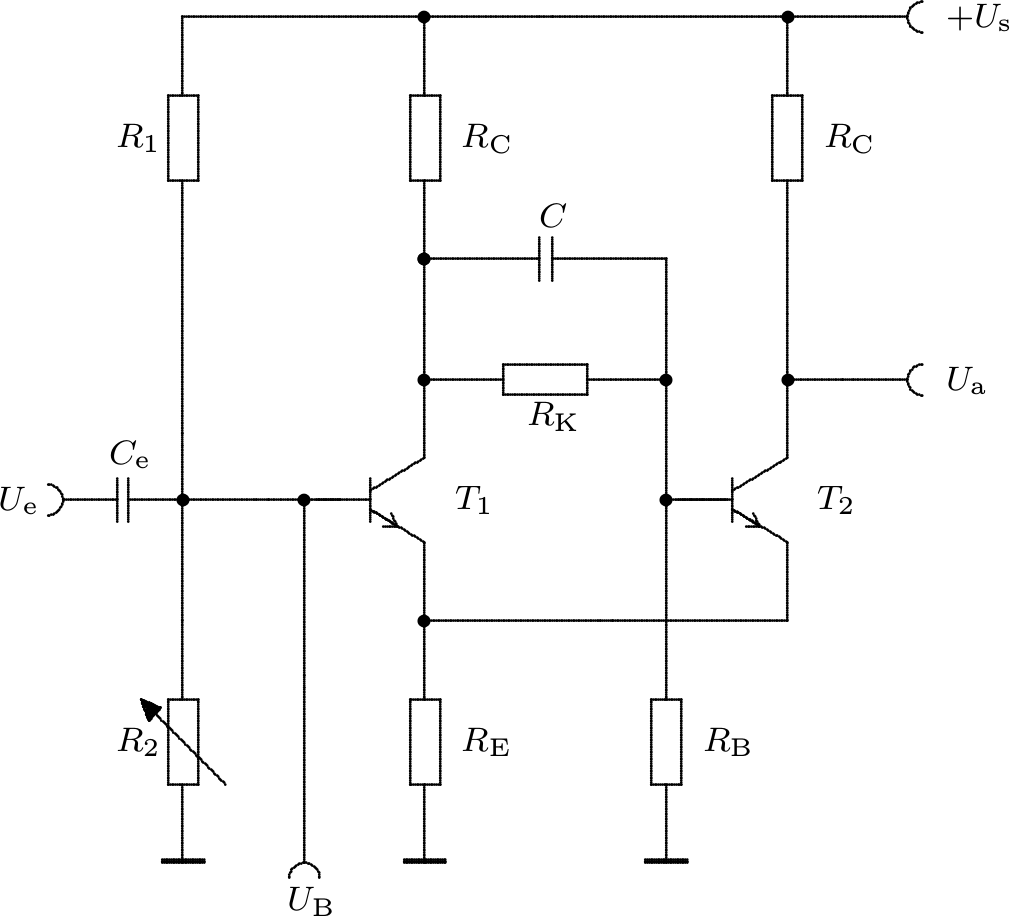
\includegraphics[width=\textwidth]{schaltskizze_st1.png}
\caption{Schaltung mit Modifizierungen $C$, $C\ix{e}$ sowie $R_1$ und $R_2$}
\end{subfigure}
\caption{Schaltbilder zum Schmitt-Trigger}
\end{figure}
\subsection{Dimensionierung}
\section{Durchführung}
\subsection{Messgeräte}
\subsection{Oszillogramme}
\section{Auswertung}
\section{Anhang}
Die originalen Messwert-Aufzeichnungen liegen bei.
\end{document}